%-------------------------------------------------------
% IIIIIII   FFFFFFFFF   PPPPPP      EEEEEEE
%   II      FF          PP   PP     EE
%   II      FFFFFF      PPPPPP      EEEE
%   II      FF          PP          EE
% IIIII     FF          PP          EEEEEEE
%--------------------------------------------------------


% Instituto Federal de Pernambuco - Campus Recife
% Departamento de Engenharia Mecânica
% Desenvolvido por Thiago Barros
% Modelo de Relatório em LaTex Para Trabalhos Acadêmicos - e Trabalho de Conclusão de Curso
% --------------------------------------------------------------------------------------------


% Estrutura do Documento

%               Arquivo main.tex - arquivo principal com as seções de cada texto
% 
%             /TCC_IFPE/
%                       /00_CONF - Contém o Arquivo de Listagem de Pacotes Para o Programa
%                       /01_PRE - Arquivos de Elementos Pré Textuais
%                       /02_TEXTO - Arquivos de Elementos Textuais (Intro;Fundamentação;  Metodo; Metodologia; Resultados e Conclusão)
%                       /03_POS- Arquivos de Elementos Pós Textuais 
%                       /04_ANEXOS - Pasta para Colocação de Arquivos para Serem Anexados
%                       /05_BIBLIOGRAFIAS- Arquivo referencia.bib para referencias
%                       /06_IMAGENS - Pasta Para Arquivamento de Imagens

% -------------------------------------------------------------------------------------------


\documentclass[a4paper,12pt,oneside]{article}

  % Pacotes Usaodos Para a Compilação do Documento

% Instituto Federal de Pernambuco - Campus Recife
% Departamento de Engenharia Mecânica
% LaTeX - 3.14
% Desenvolvido por Thiago Barros
% Modelo de Relatório em LaTex Para Trabalhos Acadêmicos - e Trabalho de Conclusão de Curso

% Lista de Pacotes


\usepackage[utf8]{inputenc}  % Permite a entrada de caracteres UTF-8 (acentos, etc.)
\usepackage[left=3cm,top=3cm,right=2cm,bottom=2cm]{geometry}  % Define as margens do documento
\usepackage[brazil]{babel}  % Localização e hifenização para o português do Brasil
\usepackage{graphicx}  % Permite a inclusão de figuras
\usepackage{amsmath}  % Pacote matemático da AMS (American Mathematical Society)
\usepackage{amsfonts}  % Fontes matemáticas da AMS
\usepackage{amssymb}  % Símbolos matemáticos da AMS
\usepackage{mathtools}  % Extensão do pacote amsmath com melhorias
\usepackage{indentfirst}  % Adiciona recuo no primeiro parágrafo de cada seção
\usepackage{ragged2e}  % Fornece o comando \justify para justificar texto
\usepackage{caption}  % Personaliza a formatação de legendas de figuras e tabelas
\usepackage{pdfpages}  % Permite a inclusão de páginas PDF externas

\usepackage{fancyhdr}  % Personaliza cabeçalhos e rodapés do documento
\pagestyle{fancy}
\fancyhf{}
\renewcommand{\headrulewidth}{0pt}
\rhead[R]{\thepage}


% Fonte Arial
%\usepackage{uarial} % Use a fonte Arial
%\renewcommand{\familydefault}{\sfdefault} 


% Fonte Times New Roman
\usepackage{times}  % Usa a fonte Times New Roman



\usepackage{lipsum} % Para gerar texto de exemplo
\usepackage{enumerate}  % Personaliza a numeração de listas enumeradas
\usepackage[skins,theorems]{tcolorbox}  % Permite a criação de caixas de texto personalizadas
\usepackage{cancel}  % Permite cancelar (barrar) termos em equações
\usepackage{listings}  % Permite a inclusão de códigos fonte de várias linguagens
\usepackage{color}  % Fornece cores para usar em documentos

\usepackage{microtype}  % Melhora o ajuste e o espaçamento de caracteres
\usepackage{tabularx}  % Extensão do ambiente tabular com larguras automáticas
\usepackage{titlesec}  % Personaliza títulos de seções, capítulos, etc.
%\usepackage{tocbibind}  % Adiciona a tabela de conteúdos, lista de figuras, etc., ao índice
\usepackage{siunitx}  % Permite a formatação fácil de unidades SI
\usepackage{physics}  % Fornece comandos úteis para notação física e matemática
\usepackage{tikz}  % Pacote para criar gráficos vetoriais
\usepackage[outline]{contour}  % Adiciona contornos a texto
\usepackage{setspace}  % Controla o espaçamento entre linhas

  \begin{document}

    % Instituto Federal de Pernambuco - Campus Recife
% Departamento de Engenharia Mecânica
% LaTeX - 3.14
% Desenvolvido por Thiago Barros
% Modelo de Relatório em LaTex Para Trabalhos Acadêmicos - e Trabalho de Conclusão de Curso
% --------------------------------------------------------------------------------------------

% Arquivo de Configuração de Titulos - Formato ABNT

\titleformat{\section}
  {\large\bfseries} % Formato da seção
  {\thesection} % Número da seção
  {1em} % Espaçamento entre o número e o título
  {} % Código antes do título
  \fontsize{12}{14}
\titleformat{\subsection}
  {\large\bfseries} % Formato da subseção
  {\thesubsection} % Número da subseção
  {1em} % Espaçamento entre o número e o título
  {} % Código antes do título
  \fontsize{12}{14}

\setstretch{1.5}

    % Elementos Pré Textuais

    \begin{center}
	
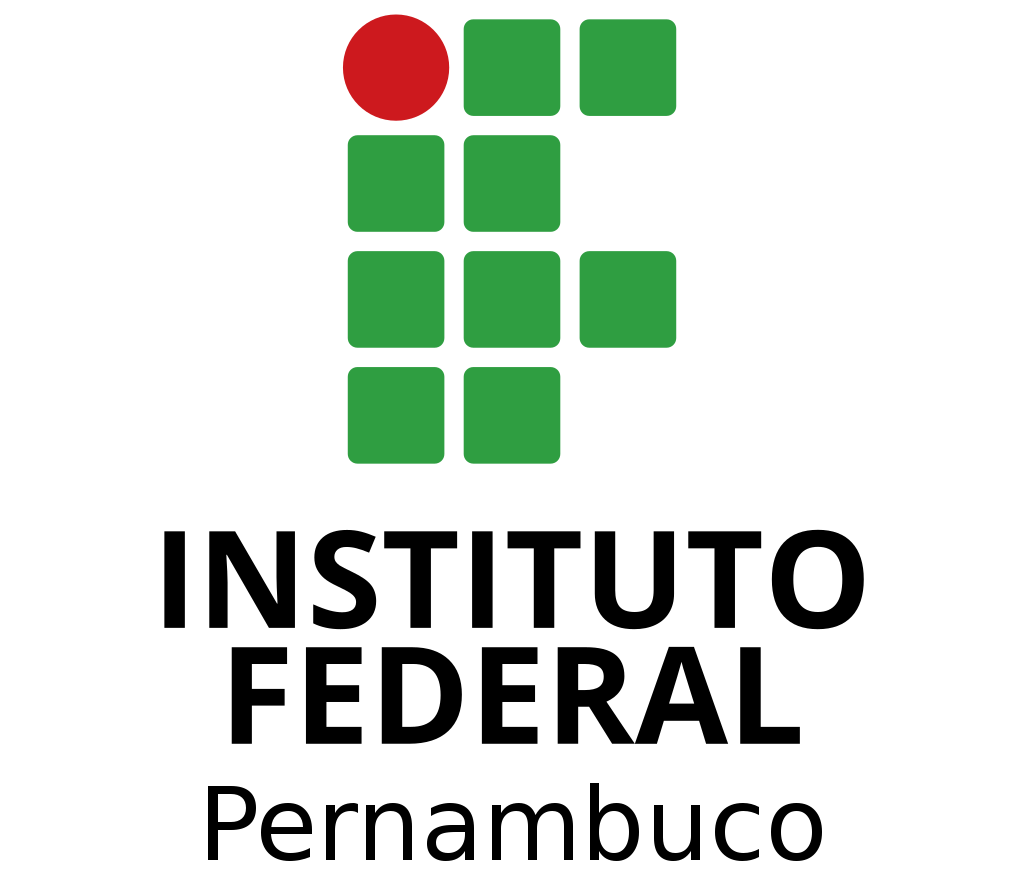
\includegraphics[width=3.5cm,height=3cm]{00_CONF/00_logo.png}

\vspace{1ex}

INSTITUTO FEDERAL DE CIÊNCIA E TECNOLOGIA DE PERNAMBUCO

Campus Recife

Coordenação Acadêmica do Curso Superior em Engenharia Mecânica

Bacharelado em Engenharia Mecânica

\vspace{3cm}

SEU NOME EM CAIXA ALTA

\vspace{3cm}

\textbf{TITULO DO TRABALHO EM CAIXA ALTA}

\vfill{}

Recife

2024


\thispagestyle{empty}
\end{center} % Elemento Obrigatório
    \begin{center}
	
	NOME COMPLETO EM CAIXA ALTA

	\vspace{6cm}

	\textbf{TITULO DO TRABALHO EM CAIXA ALTA}
	
\end{center}

\vspace{1cm}

	\hfill\begin{minipage}{0.5\linewidth}
		{Trabalho de conclusão de curso apresentado a Coordenação da Graduação do Curso Superior do Bacharelado Engenharia Mecânica, do Instituto Federal de Ciência e Tecnologia de Pernambuco, como requisito para obtenção de título de Bacharel em Engenharia Mecânica.
		
		Orientador: Prof. Dr. Nome do Orientador
	
		%Corientador: Prof. Dr. Nome do Corientador % - Caso Exista

		}

\end{minipage}

\vfill{}

\begin{center}

	Recife

	\vspace{0.2cm}

	2024

\end{center}

\thispagestyle{empty}
 % Elemento Obrigatório
    FICHA CATALOGRAFICA
ESSA PÁGINA ESTÁ EM BRANCO - SOLICITE A FICHA CATALOGRÁFICA PARA COLOCAR NO TEXTO
\thispagestyle{empty} % Elemento Obrigatório
    \vspace*{\fill} 
\begin{center}

    \vspace{10cm}
    
    \textbf{TITUTO DO TRABALHO EM CAIXA ALTA}

    Trabalho Aprovado, Recife, Data de APROVAÇÃO

    \hspace{3cm}


    \rule{12cm}{0.2mm}

    Professor Orientador

    \hspace{3cm}

    \rule{12cm}{0.2mm}

    Professor Orientador

    \hspace{3cm}

    \rule{12cm}{0.2mm}

    Professor Orientador

    \hspace{3cm}

    
    \vfill{}

    Recife

    2024

\end{center}
\thispagestyle{empty} % Elemento Obrigatório

    \vspace*{\fill} 
\vfill{}
\begin{flushright}

    Aos meus pais. Pela paciência e suporte nessa jornada difícil.

\end{flushright}

\thispagestyle{empty}  % Elemento Opcional
    \begin{center}
    \textbf{AGRADECIMENTOS}
 \end{center}
 
 \hspace{2cm}
 
 \begin{center}
     
    Gostaria de expressar meus sinceros agradecimentos a todas as pessoas que contribuíram para este trabalho. Em particular, gostaria de agradecer ao meu orientador pelo apoio e orientação ao longo deste processo. Também gostaria de agradecer à minha família e amigos pelo seu apoio contínuo e incentivo. Por fim, gostaria de agradecer à instituição pela oportunidade de realizar este trabalho e pelo suporte fornecido. 


 \end{center}
 
 \thispagestyle{empty} % Elemento Opcional
    \vspace*{\fill} 
\vfill{}
\begin{flushright}

    "Você não pode gerenciar o que não pode medir." - William Edwards Deming
    
\end{flushright}

\thispagestyle{empty} % Elemento Opcional

    \begin{center}
   \textbf{RESUMO}
\end{center}

\hspace{2cm}

\begin{justify}
    
    Modelo modelo modelo modelo modelo modelo modelo modelo modelo modelo modelo modelo modelo modelo modelo modelo modelo modelo modelo modelo modelo modelo modelo modelo modelo modelo modelo modelo modelo modelo modelo modelo modelo modelo modelo modelo modelo modelo modelo modelo modelo modelo modelo modelo modelo modelo modelo modelo modelo modelo modelo modelo modelo modelo modelo modelo modelo modelo modelo modelo modelo modelo modelo modelo modelo modelo modelo modelo modelo modelo modelo modelo modelo modelo modelo modelo modelo modelo modelo modelo modelo modelo modelo modelo modelo.\\

    \textbf{Palavras Chave: Batata,Batata}

\end{justify}

\thispagestyle{empty} % Elemento Obrigatório
    \begin{center}
	\textbf{ABSTRACT}
 \end{center}
 
 \hspace{2cm}
 
 \begin{justify}
	
	Potato Potato Potato PotatoPotato PotatoPotato PotatoPotato PotatoPotato PotatoPotato Potato
	Potato Potato Potato PotatoPotato PotatoPotato PotatoPotato PotatoPotato PotatoPotato Potato
	Potato Potato Potato PotatoPotato PotatoPotato PotatoPotato PotatoPotato PotatoPotato Potato
	Potato Potato Potato PotatoPotato PotatoPotato PotatoPotato PotatoPotato PotatoPotato Potato
	Potato Potato Potato PotatoPotato PotatoPotato PotatoPotato PotatoPotato PotatoPotato Potato
	Potato Potato Potato PotatoPotato PotatoPotato PotatoPotato PotatoPotato PotatoPotato Potato\\

	 \textbf{Keywords: pOTATO. pOTATO, Potato}

 \end{justify}
 
 \thispagestyle{empty} % Elemento Obrigatório


    \renewcommand{\listfigurename}{}
\begin{center}
	\textbf{LISTA DE FIGURAS}
 \end{center}
\listoffigures
\thispagestyle{empty}
\pagebreak
\clearpage % Elemento Opcional
    \renewcommand{\listtablename}{}
\begin{center}
	\textbf{LISTA DE TABELAS}
 \end{center}
\listoftables
\thispagestyle{empty}
\pagebreak
\clearpage % Elemento Opcional
    \begin{center}
	\textbf {LISTA DE SIGLAS}
\end{center}
\vspace{0.5cm}
\begin{flushleft}

	\begin{tabularx}{12cm}{X X l}
		$\dot{Q}$ &  &  \itshape Fluxo de Calor\\
		$K$ &  &  \itshape Condutividade Térmica\\
		$C_{p}$ &  &  \itshape Calor Específico\\
		$\dot{m}$ &  &  \itshape Vazão mássica\\
		$\epsilon$ &  &  \itshape Efetividade
		
	\end{tabularx}
\end{flushleft}
\thispagestyle{empty} % Elemento Opcional
    \begin{center}
	\textbf {LISTA DE SÍMBOLOS}
\end{center}
\vspace{0.5cm}
\begin{flushleft}
	\begin{tabularx}{12cm}{X X l}
	
		$\dot{Q}$ &  &  \itshape Fluxo de Calor\\
		$K$ &  &  \itshape Condutividade Térmica\\
		$C_{p}$ &  &  \itshape Calor Específico\\
		$\dot{m}$ &  &  \itshape Vazão mássica\\
		$\epsilon$ &  &  \itshape Efetividade

	\end{tabularx}
\end{flushleft}
\thispagestyle{empty} % Elemento Opcional

    \begin{center}
	\textbf {SUMÁRIO}
\end{center}

\renewcommand{\contentsname}{}\tableofcontents
\thispagestyle{empty}
 % Elemento Obrigatório

    %--------------------------------------------------------------------

    % Elementos Textuais

    \begin{flushright}
\justify
\titleformat{\section}{\large\bfseries}{\thesection}{1em}{}
\section{INTRODUÇÃO}
\vspace{0.5cm}

Batata Batata Batata Batata Batata Batata Batata Batata Batata Batata Batata Batata 
Batata Batata Batata Batata Batata Batata Batata Batata Batata Batata Batata Batata 
Batata Batata Batata Batata Batata Batata Batata Batata Batata Batata Batata Batata 
Batata Batata Batata Batata Batata Batata Batata Batata Batata Batata Batata Batata 
Batata Batata Batata Batata Batata Batata Batata Batata Batata Batata Batata Batata 
Batata Batata Batata Batata Batata Batata Batata Batata Batata Batata Batata Batata 
Batata Batata Batata Batata Batata Batata Batata Batata Batata Batata Batata Batata 
Batata Batata Batata Batata Batata Batata Batata Batata Batata Batata Batata Batata 
Batata Batata Batata Batata Batata Batata Batata Batata Batata Batata Batata Batata 
Batata Batata Batata Batata Batata Batata Batata Batata Batata Batata Batata Batata 
Batata Batata Batata Batata Batata Batata Batata Batata Batata Batata Batata Batata 
Batata Batata Batata Batata Batata Batata Batata Batata Batata Batata Batata Batata 
Batata Batata Batata Batata Batata Batata Batata Batata Batata Batata Batata Batata 
Batata Batata Batata Batata Batata Batata Batata Batata Batata Batata Batata Batata 
Batata Batata Batata Batata Batata Batata Batata Batata Batata Batata Batata Batata 
Batata Batata Batata Batata Batata Batata Batata Batata Batata Batata Batata Batata 
Batata Batata Batata Batata Batata Batata Batata Batata Batata Batata Batata Batata 
Batata Batata Batata Batata Batata Batata Batata Batata Batata Batata Batata Batata 
Batata Batata Batata Batata Batata Batata Batata Batata Batata Batata Batata Batata 
Batata Batata Batata Batata Batata Batata Batata Batata Batata Batata Batata Batata 
Batata Batata Batata Batata Batata Batata Batata Batata Batata Batata Batata Batata 
Batata Batata Batata Batata Batata Batata Batata Batata Batata Batata Batata Batata 
Batata Batata Batata Batata Batata Batata Batata Batata Batata Batata Batata Batata 

Batata Batata Batata Batata Batata Batata Batata Batata Batata Batata Batata Batata 
Batata Batata Batata Batata Batata Batata Batata Batata Batata Batata Batata Batata 
Batata Batata Batata Batata Batata Batata Batata Batata Batata Batata Batata Batata 
Batata Batata Batata Batata Batata Batata Batata Batata Batata Batata Batata Batata 
Batata Batata Batata Batata Batata Batata Batata Batata Batata Batata Batata Batata 
Batata Batata Batata Batata Batata Batata Batata Batata Batata Batata Batata Batata 
Batata Batata Batata Batata Batata Batata Batata Batata Batata Batata Batata Batata 
Batata Batata Batata Batata Batata Batata Batata Batata Batata Batata Batata Batata 
Batata Batata Batata Batata Batata Batata Batata Batata Batata Batata Batata Batata 
Batata Batata Batata Batata Batata Batata Batata Batata Batata Batata Batata Batata 

\end{flushright}

    \begin{flushright}

    \justify

    \titleformat{\section}{\large\bfseries}{\thesection}{1em}{}
    \titleformat{\subsection}{\normalfont\large}{\thesubsection}{1em}{}

    \section{FUNDAMENTAÇÃO TEÓRICA}
    \vspace{0.5cm}
    \subsection{BATATA}
    \vspace{0.5cm}   

    Batata Batata Batata Batata Batata Batata Batata Batata Batata Batata Batata Batata 
    Batata Batata Batata Batata Batata Batata Batata Batata Batata Batata Batata Batata 
    Batata Batata Batata Batata Batata Batata Batata Batata Batata Batata Batata Batata 
    Batata Batata Batata Batata Batata Batata Batata Batata Batata Batata Batata Batata 
    Batata Batata Batata Batata Batata Batata Batata Batata Batata Batata Batata Batata 
    Batata Batata Batata Batata Batata Batata Batata Batata Batata Batata Batata Batata 
    Batata Batata Batata Batata Batata Batata Batata Batata Batata Batata Batata Batata 
    Batata Batata Batata Batata Batata Batata Batata Batata Batata Batata Batata Batata 
    Batata Batata Batata Batata Batata Batata Batata Batata Batata Batata Batata Batata 
    Batata Batata Batata Batata Batata Batata Batata Batata Batata Batata Batata Batata 
    Batata Batata Batata Batata Batata Batata Batata Batata Batata Batata Batata Batata 
    Batata Batata Batata Batata Batata Batata Batata Batata Batata Batata Batata Batata 
    Batata Batata Batata Batata Batata Batata Batata Batata Batata Batata Batata Batata 
    Batata Batata Batata Batata Batata Batata Batata Batata Batata Batata Batata Batata 
    Batata Batata Batata Batata Batata Batata Batata Batata Batata Batata Batata Batata 
    Batata Batata Batata Batata Batata Batata Batata Batata Batata Batata Batata Batata 
    Batata Batata Batata Batata Batata Batata Batata Batata Batata Batata Batata Batata 
    Batata Batata Batata Batata Batata Batata Batata Batata Batata Batata Batata Batata 
    Batata Batata Batata Batata Batata Batata Batata Batata Batata Batata Batata Batata 
    Batata Batata Batata Batata Batata Batata Batata Batata Batata Batata Batata Batata 
    Batata Batata Batata Batata Batata Batata Batata Batata Batata Batata Batata Batata 
    Batata Batata Batata Batata Batata Batata Batata Batata Batata Batata Batata Batata 
    Batata Batata Batata Batata Batata Batata Batata Batata Batata Batata Batata Batata 
    
    Batata Batata Batata Batata Batata Batata Batata Batata Batata Batata Batata Batata 
    Batata Batata Batata Batata Batata Batata Batata Batata Batata Batata Batata Batata 
    Batata Batata Batata Batata Batata Batata Batata Batata Batata Batata Batata Batata 
    Batata Batata Batata Batata Batata Batata Batata Batata Batata Batata Batata Batata 
    Batata Batata Batata Batata Batata Batata Batata Batata Batata Batata Batata Batata 
    Batata Batata Batata Batata Batata Batata Batata Batata Batata Batata Batata Batata 
    Batata Batata Batata Batata Batata Batata Batata Batata Batata Batata Batata Batata 
    Batata Batata Batata Batata Batata Batata Batata Batata Batata Batata Batata Batata 
    Batata Batata Batata Batata Batata Batata Batata Batata Batata Batata Batata Batata 
    Batata Batata Batata Batata Batata Batata Batata Batata Batata Batata Batata Batata \\

    \begin{equation}
        P = \frac{F}{A} 
    \end{equation}\\

    \begin{equation}
        F = P \times A
    \end{equation}\\

\end{flushright}
    \begin{flushright}

    \justify

    \titleformat{\section}{\large\bfseries}{\thesection}{1em}{}
    \titleformat{\subsection}{\normalfont\large}{\thesubsection}{1em}{}

    \section{METODOLOGIA}
    \vspace{0.5cm}
 
    Batata Batata Batata Batata Batata Batata Batata Batata Batata Batata Batata Batata 
    Batata Batata Batata Batata Batata Batata Batata Batata Batata Batata Batata Batata 
    Batata Batata Batata Batata Batata Batata Batata Batata Batata Batata Batata Batata 
    Batata Batata Batata Batata Batata Batata Batata Batata Batata Batata Batata Batata 
    Batata Batata Batata Batata Batata Batata Batata Batata Batata Batata Batata Batata 
    Batata Batata Batata Batata Batata Batata Batata Batata Batata Batata Batata Batata 
    Batata Batata Batata Batata Batata Batata Batata Batata Batata Batata Batata Batata 
    Batata Batata Batata Batata Batata Batata Batata Batata Batata Batata Batata Batata 
    Batata Batata Batata Batata Batata Batata Batata Batata Batata Batata Batata Batata 
    Batata Batata Batata Batata Batata Batata Batata Batata Batata Batata Batata Batata 
    Batata Batata Batata Batata Batata Batata Batata Batata Batata Batata Batata Batata 
    Batata Batata Batata Batata Batata Batata Batata Batata Batata Batata Batata Batata 
    Batata Batata Batata Batata Batata Batata Batata Batata Batata Batata Batata Batata 
    Batata Batata Batata Batata Batata Batata Batata Batata Batata Batata Batata Batata 
    Batata Batata Batata Batata Batata Batata Batata Batata Batata Batata Batata Batata 
    Batata Batata Batata Batata Batata Batata Batata Batata Batata Batata Batata Batata 
    Batata Batata Batata Batata Batata Batata Batata Batata Batata Batata Batata Batata 
    Batata Batata Batata Batata Batata Batata Batata Batata Batata Batata Batata Batata 
    Batata Batata Batata Batata Batata Batata Batata Batata Batata Batata Batata Batata 
    Batata Batata Batata Batata Batata Batata Batata Batata Batata Batata Batata Batata 
    Batata Batata Batata Batata Batata Batata Batata Batata Batata Batata Batata Batata 
    Batata Batata Batata Batata Batata Batata Batata Batata Batata Batata Batata Batata 
    Batata Batata Batata Batata Batata Batata Batata Batata Batata Batata Batata Batata 
    
    Batata Batata Batata Batata Batata Batata Batata Batata Batata Batata Batata Batata 
    Batata Batata Batata Batata Batata Batata Batata Batata Batata Batata Batata Batata 
    Batata Batata Batata Batata Batata Batata Batata Batata Batata Batata Batata Batata 
    Batata Batata Batata Batata Batata Batata Batata Batata Batata Batata Batata Batata 
    Batata Batata Batata Batata Batata Batata Batata Batata Batata Batata Batata Batata 
    Batata Batata Batata Batata Batata Batata Batata Batata Batata Batata Batata Batata 
    Batata Batata Batata Batata Batata Batata Batata Batata Batata Batata Batata Batata 
    Batata Batata Batata Batata Batata Batata Batata Batata Batata Batata Batata Batata 
    Batata Batata Batata Batata Batata Batata Batata Batata Batata Batata Batata Batata 
    Batata Batata Batata Batata Batata Batata Batata Batata Batata Batata Batata Batata 
    
\end{flushright}
    \section{ANÁLISE DE RESULTADOS}
\vspace{0.5cm}

Batata Batata Batata Batata Batata Batata Batata Batata Batata Batata Batata Batata 
    Batata Batata Batata Batata Batata Batata Batata Batata Batata Batata Batata Batata 
    Batata Batata Batata Batata Batata Batata Batata Batata Batata Batata Batata Batata 
    Batata Batata Batata Batata Batata Batata Batata Batata Batata Batata Batata Batata 
    Batata Batata Batata Batata Batata Batata Batata Batata Batata Batata Batata Batata 
    Batata Batata Batata Batata Batata Batata Batata Batata Batata Batata Batata Batata 
    Batata Batata Batata Batata Batata Batata Batata Batata Batata Batata Batata Batata 
    Batata Batata Batata Batata Batata Batata Batata Batata Batata Batata Batata Batata 
    Batata Batata Batata Batata Batata Batata Batata Batata Batata Batata Batata Batata 
    Batata Batata Batata Batata Batata Batata Batata Batata Batata Batata Batata Batata 
    Batata Batata Batata Batata Batata Batata Batata Batata Batata Batata Batata Batata 
    Batata Batata Batata Batata Batata Batata Batata Batata Batata Batata Batata Batata 
    Batata Batata Batata Batata Batata Batata Batata Batata Batata Batata Batata Batata 
    Batata Batata Batata Batata Batata Batata Batata Batata Batata Batata Batata Batata 
    Batata Batata Batata Batata Batata Batata Batata Batata Batata Batata Batata Batata 
    Batata Batata Batata Batata Batata Batata Batata Batata Batata Batata Batata Batata 
    Batata Batata Batata Batata Batata Batata Batata Batata Batata Batata Batata Batata 
    Batata Batata Batata Batata Batata Batata Batata Batata Batata Batata Batata Batata 
    Batata Batata Batata Batata Batata Batata Batata Batata Batata Batata Batata Batata 
    Batata Batata Batata Batata Batata Batata Batata Batata Batata Batata Batata Batata 
    Batata Batata Batata Batata Batata Batata Batata Batata Batata Batata Batata Batata 
    Batata Batata Batata Batata Batata Batata Batata Batata Batata Batata Batata Batata 
    Batata Batata Batata Batata Batata Batata Batata Batata Batata Batata Batata Batata 
    
    Batata Batata Batata Batata Batata Batata Batata Batata Batata Batata Batata Batata 
    Batata Batata Batata Batata Batata Batata Batata Batata Batata Batata Batata Batata 
    Batata Batata Batata Batata Batata Batata Batata Batata Batata Batata Batata Batata 
    Batata Batata Batata Batata Batata Batata Batata Batata Batata Batata Batata Batata 
    Batata Batata Batata Batata Batata Batata Batata Batata Batata Batata Batata Batata 
    Batata Batata Batata Batata Batata Batata Batata Batata Batata Batata Batata Batata 
    Batata Batata Batata Batata Batata Batata Batata Batata Batata Batata Batata Batata 
    Batata Batata Batata Batata Batata Batata Batata Batata Batata Batata Batata Batata 
    Batata Batata Batata Batata Batata Batata Batata Batata Batata Batata Batata Batata 
    Batata Batata Batata Batata Batata Batata Batata Batata Batata Batata Batata Batata 

    \section{CONSIDERAÇÕES}
\vspace{0.5cm}

Batata Batata Batata Batata Batata Batata Batata Batata Batata Batata Batata Batata 
    Batata Batata Batata Batata Batata Batata Batata Batata Batata Batata Batata Batata 
    Batata Batata Batata Batata Batata Batata Batata Batata Batata Batata Batata Batata 
    Batata Batata Batata Batata Batata Batata Batata Batata Batata Batata Batata Batata 
    Batata Batata Batata Batata Batata Batata Batata Batata Batata Batata Batata Batata 
    Batata Batata Batata Batata Batata Batata Batata Batata Batata Batata Batata Batata 
    Batata Batata Batata Batata Batata Batata Batata Batata Batata Batata Batata Batata 
    Batata Batata Batata Batata Batata Batata Batata Batata Batata Batata Batata Batata 
    Batata Batata Batata Batata Batata Batata Batata Batata Batata Batata Batata Batata 
    Batata Batata Batata Batata Batata Batata Batata Batata Batata Batata Batata Batata 
    Batata Batata Batata Batata Batata Batata Batata Batata Batata Batata Batata Batata 
    Batata Batata Batata Batata Batata Batata Batata Batata Batata Batata Batata Batata 
    Batata Batata Batata Batata Batata Batata Batata Batata Batata Batata Batata Batata 
    Batata Batata Batata Batata Batata Batata Batata Batata Batata Batata Batata Batata 
    Batata Batata Batata Batata Batata Batata Batata Batata Batata Batata Batata Batata 
    Batata Batata Batata Batata Batata Batata Batata Batata Batata Batata Batata Batata 
    Batata Batata Batata Batata Batata Batata Batata Batata Batata Batata Batata Batata 
    Batata Batata Batata Batata Batata Batata Batata Batata Batata Batata Batata Batata 
    Batata Batata Batata Batata Batata Batata Batata Batata Batata Batata Batata Batata 
    Batata Batata Batata Batata Batata Batata Batata Batata Batata Batata Batata Batata 
    Batata Batata Batata Batata Batata Batata Batata Batata Batata Batata Batata Batata 
    Batata Batata Batata Batata Batata Batata Batata Batata Batata Batata Batata Batata 
    Batata Batata Batata Batata Batata Batata Batata Batata Batata Batata Batata Batata 
    
    Batata Batata Batata Batata Batata Batata Batata Batata Batata Batata Batata Batata 
    Batata Batata Batata Batata Batata Batata Batata Batata Batata Batata Batata Batata 
    Batata Batata Batata Batata Batata Batata Batata Batata Batata Batata Batata Batata 
    Batata Batata Batata Batata Batata Batata Batata Batata Batata Batata Batata Batata 
    Batata Batata Batata Batata Batata Batata Batata Batata Batata Batata Batata Batata 
    Batata Batata Batata Batata Batata Batata Batata Batata Batata Batata Batata Batata 
    Batata Batata Batata Batata Batata Batata Batata Batata Batata Batata Batata Batata 
    Batata Batata Batata Batata Batata Batata Batata Batata Batata Batata Batata Batata 
    Batata Batata Batata Batata Batata Batata Batata Batata Batata Batata Batata Batata 
    Batata Batata Batata Batata Batata Batata Batata Batata Batata Batata Batata Batata 


    % Elementos Pós Textuais

    \section*{REFERÊNCIAS}
\addcontentsline{toc}{section}{REFERÊNCIAS}
\vspace{0.5cm}

%\bibliographystyle{plain} 
%\bibliography{bibliografia}


 % Elemento Opcional

    %\section*{REFERÊNCIAS}
\addcontentsline{toc}{section}{REFERÊNCIAS}
\vspace{0.5cm}


\textbf{BOSCH}, RE25850 - Pressure relief valve, pilot-operated Type DB; DBW - Bosch Rexroth - 2021 \\

\textbf{LINSINGEN} Von Ivan, Fundamentos de Sistemas Hidráulicos, Editora da UFSC - 2001 \\

 % Elemento Opcional
    %\section*{ANEXOS}
\addcontentsline{toc}{section}{ANEXOS}
\vspace{0.5cm}

\textbf{ANEXO 1 - CATÁLOGO BOSCH}

\includepdf[pages=-]{00_ANEXOS/ANEXO_00.pdf}  % Elemento Opcional
    %\section*{ANEXOS}
\addcontentsline{toc}{section}{ANEXOS}
\vspace{0.5cm}

\textbf{ANEXO 1 - CATÁLOGO BOSCH}

\includepdf[pages=-]{00_ANEXOS/ANEXO_00.pdf} % Elemento Opcional
    %\section*{ANEXOS}
\addcontentsline{toc}{section}{ANEXOS}
\vspace{0.5cm}

\textbf{ANEXO 1 - CATÁLOGO BOSCH}

\includepdf[pages=-]{00_ANEXOS/ANEXO_00.pdf} % Elemento Opcional

  \end{document}
